\documentclass{article}
\usepackage{lmodern}
\usepackage{graphicx} % Required for inserting images
\usepackage{caption}
%\renewcommand{\thesubsection}{\arabic{subsection}}

\title{Peer review \#2 - GC11}
\author{Samuele Pischedda, Angelo Prete, Gabriele Raveggi, Andrea Sanvito }
\date{06/05/2024}

\begin{document}

\begin{titlepage}
\maketitle
\end{titlepage}
\section*{General Overview}
In this document we describe the UML of our Codex Naturalis java implementation.
In particular, we will explain how we implemented the controller of the MVC architectural pattern and the client-server communication protocol.

\section*{Introduction}
The project has been extended by adding network functionalities.
The game uses a double connection, one for joining and leaving lobbies (the "main menu" connection) and the other one for in-game actions and for the chat.
Actions from the client to the server and updates from the model to the client have been implemented using the command pattern.
\section{Model}
In particular, the updates are generated in the model and sent to all the classes that need them through the use of the observer-observable pattern.
\begin{center}
    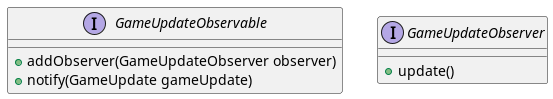
\includegraphics[scale=0.5]{pngs/observer}
\end{center}
All the model classes that produce updates must implement the \texttt{GameUpdateObservable} interface.
The \texttt{GameModel} constructor now takes a \texttt{List<GameUpdateObserver>}, so that all the \texttt{GameUpdateObservable} can register them.
\section{Network}
The network communication is implemented using classes that extend interfaces shared by both the RMI and socket implementation.
The main connection to the server (used for creating lobbies and starting games) is opened when the client is started and it
is kept alive until the client is closed.
The \texttt{RMIMainServer} and \texttt{SocketMainServer} classes, that implement the \texttt{MainServerActions} interface,
are used when the client is connecting to the server for the first time.
\begin{center}
    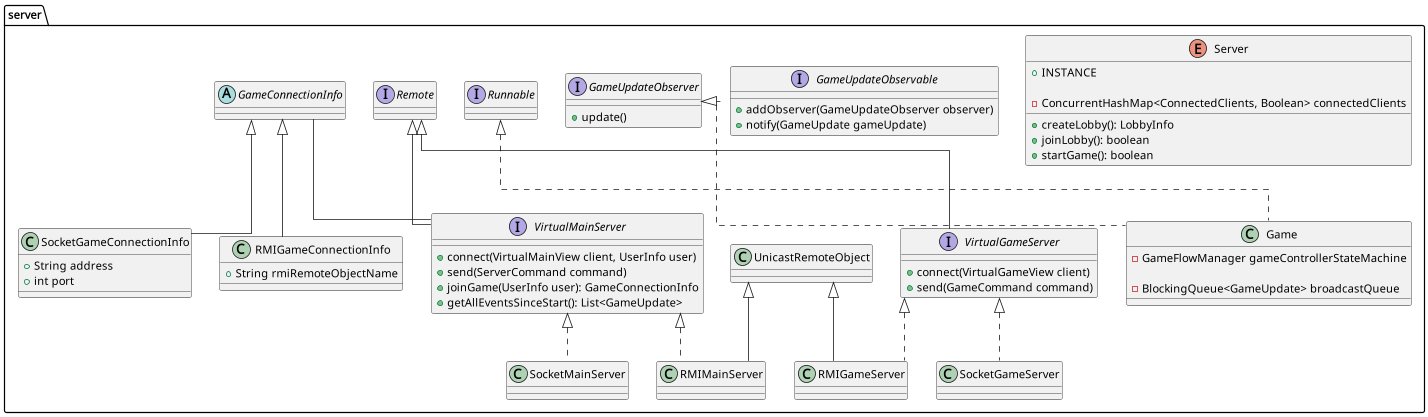
\includegraphics[scale=0.25]{pngs/server1}
\end{center}
We kept the RMI implementation trivial and made the socket implementation mimic the RMI behaviour.
Once the connection is established (via the RMI Registry or through a socket), the clients must call the \texttt{connect(...)} method
that take their \texttt{VirtualMainView} as parameter.
This interface is the client's dual of \texttt{MainServerActions} and is implemented by \texttt{RMIMainView} and \texttt{SocketMainView} classes.
The interface offers methods to show errors on the view or to send the list of updated lobbies.
\begin{center}
    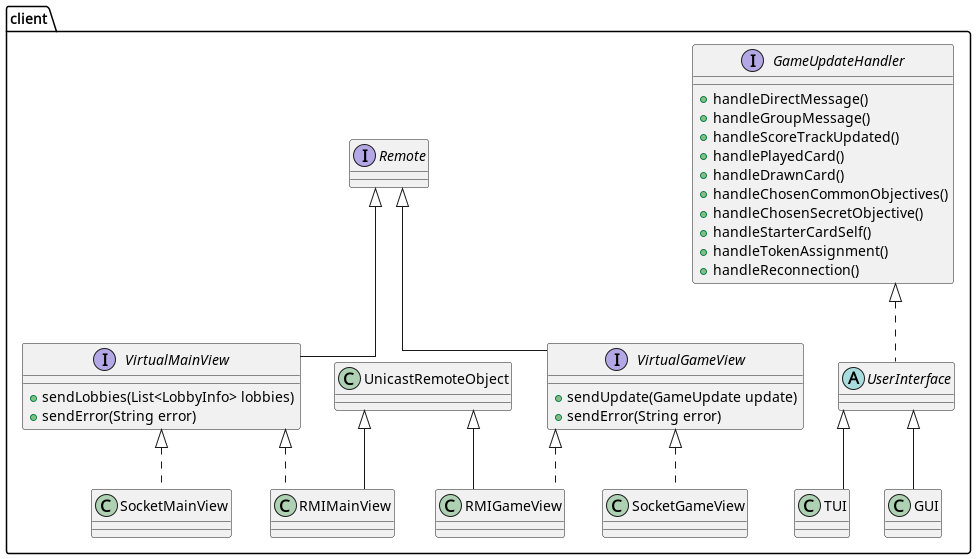
\includegraphics[scale=0.3]{pngs/client}
\end{center}
By sending a \texttt{ServerCommand} (done by calling the method on the \texttt{MainServerActions}) a client can create, join or leave a lobby.
When the client is ready he can call the \texttt{joinGame} method and receive a \texttt{ConnectionInfo} object that holds
the information needed to open the second connection.

\begin{center}
    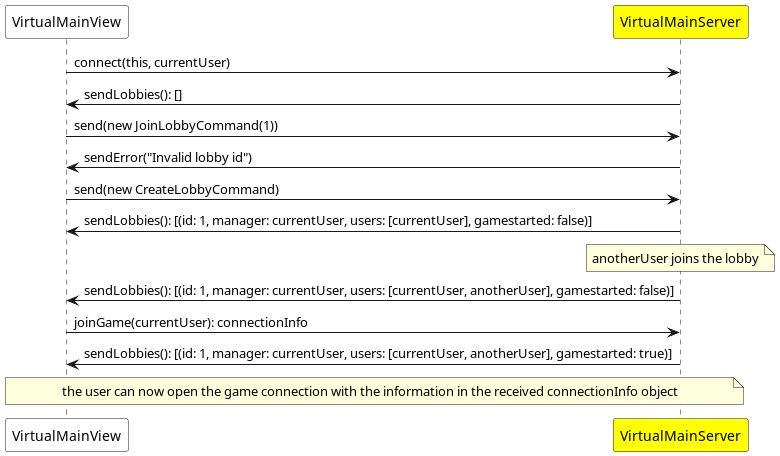
\includegraphics[scale=0.35]{pngs/sequence_game_creation}
\end{center}
The second connection has the same structure as the first: there is a\texttt{VirtualGameServer} and a \texttt{VirtualGameView}, both implemented as RMI and socket classes.
The clients can send \texttt{GameCommand} objects to the controller by calling the \texttt{send(...)} method of \texttt{VirtualGameServer}
and they can receive \texttt{GameUpdate} objects when the server calls on the \texttt{VirtualGameView}s the \texttt{sendUpdate(...)} method.
Once the clients receive the update object, they can call the \texttt{execute(...)} method on them by passing an object that implements \texttt{GameUpdateHandler} as parameter.
This makes the implementations of GUI and CLI independent, as they can simply define the \texttt{GameUpdateHandler} interface.
\begin{center}
    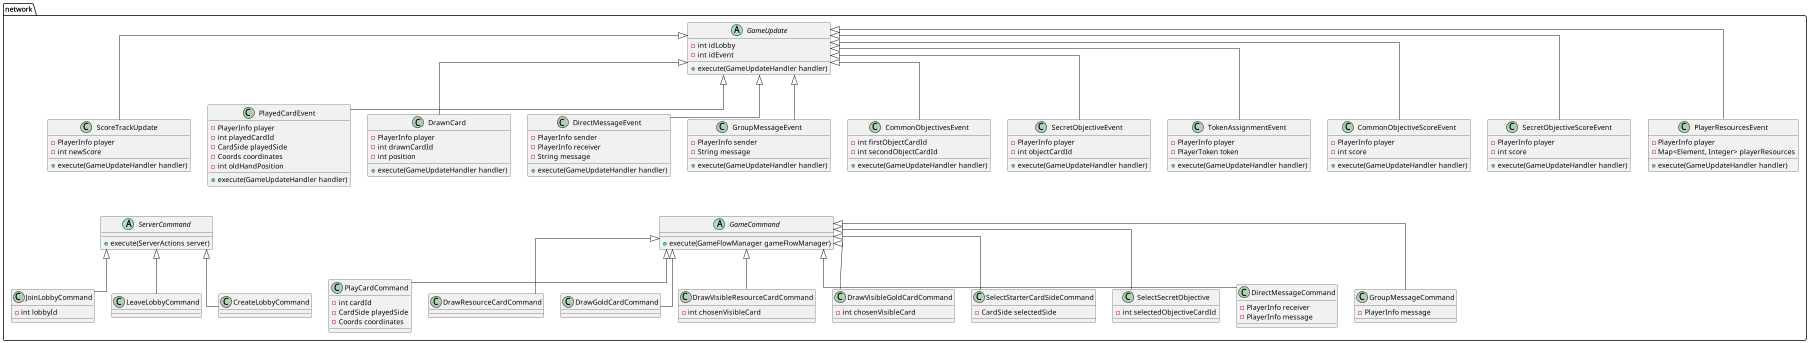
\includegraphics[scale=0.2]{pngs/network}
\end{center}

\newpage
\section{Controller}
The controller package has been updated by implementing a main controller class as a runnable, which is run by a thread started in the main server as soon as the game begins.
The class uses a state machine designed through the State Pattern. A class to update the model (\texttt{GameModelUpdater}) was added.
\begin{center}
    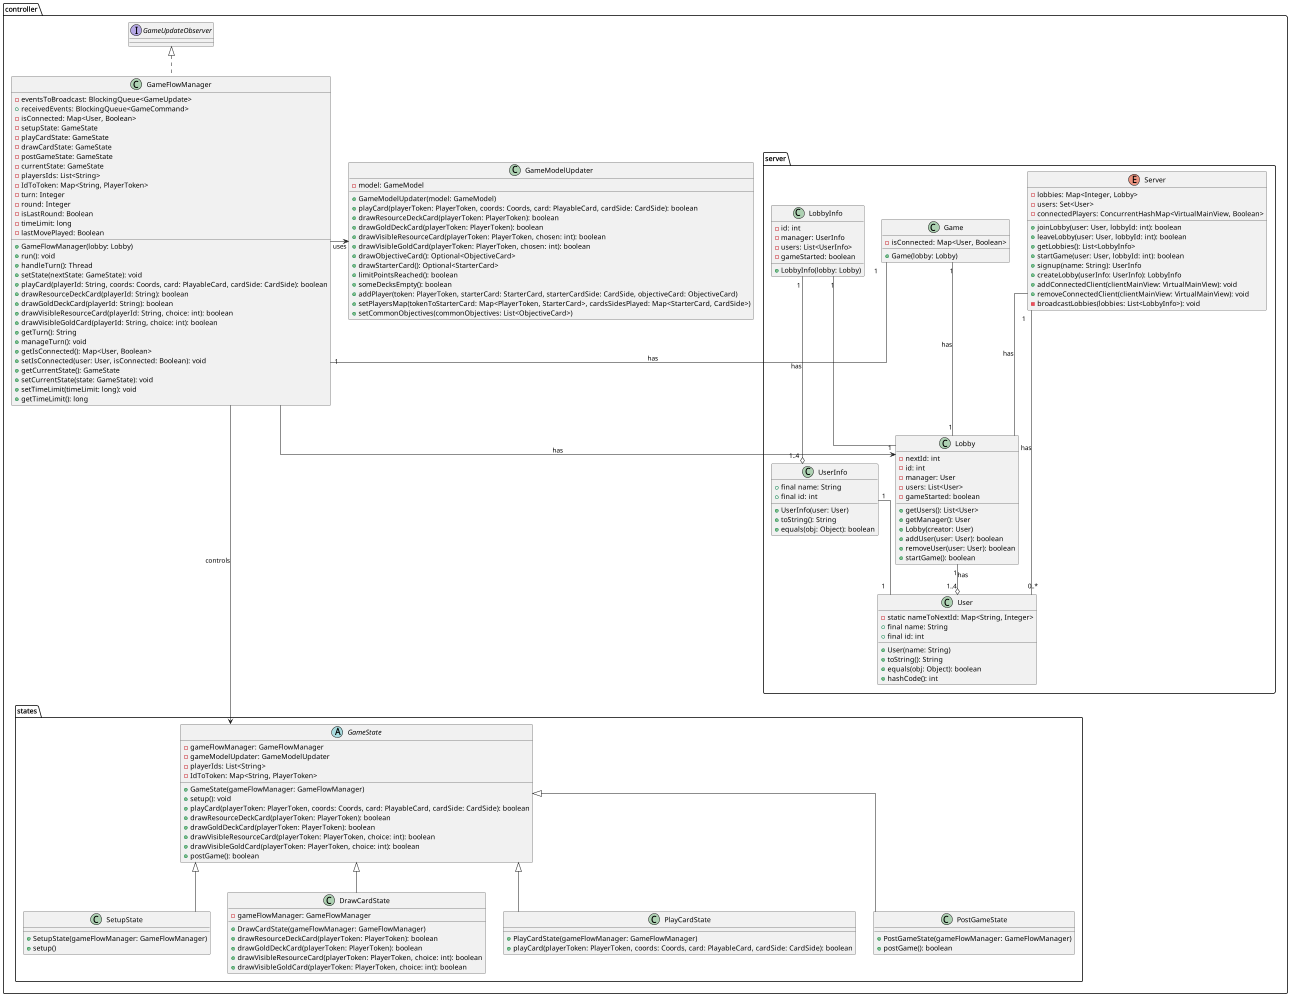
\includegraphics[scale=0.25]{pngs/controller}
\end{center}
\subsection{GameFlowManager}
This class represents the game itself. It's a runnable, whose \texttt{run()} method is divided into three main phases:
\begin{itemize}
    \item \textbf{pre-game (or setup) phase}: allows users to choose their tokens, the side to play of their starter card and the objective card.
    It also creates all entities needed for the game to happen.
    \item \textbf{in-game phase}: loops through the players' turns, starting two threads each turn: one to actually handle the turn,
        and the other to keep a timer, to forbid players from going beyond a \texttt{limitTime}.
    \item \textbf{post-game phase}: handles the final phase of the game, where the winner is declared and all clients are notified of the results.
\end{itemize}
It also keeps track of the current turn, the current round (composed by more turns), and the current player.
\subsection{GameState}
The information of the {GameFlowManager} state is kept through a bunch of \texttt{GameState} objects, following the State Pattern.
This way, players can make their moves only when the \texttt{GameFlowManager} is in the correct state.

All the methods in the abstract class \texttt{GameState} return a boolean.
By default, they return false. Each state will override its own methods.
The return value is used by the controller to understand whether the action was successful or not.
In particular, the states used are:
\begin{itemize}
    \item \texttt{SetupState:} when the \texttt{GameFlowManager} is created, its \texttt{currentState} is set to this state.
          Here, the only overridden method is \texttt{setup()}, which handles the initial part of the game.
    \item \texttt{PlayCardState}: state where a player needs to play a card. It overrides the \texttt{playCard} method;
    \item \texttt{DrawCardState}: state where a player needs to draw a card. It overrides the four \texttt{drawCard} methods;
    \item \texttt{PostGameState}: through this state, the \texttt{GameFlowManager} handles the final part of the game.
                                  It overrides the \texttt{postGame} method.
\end{itemize}
\begin{center}
    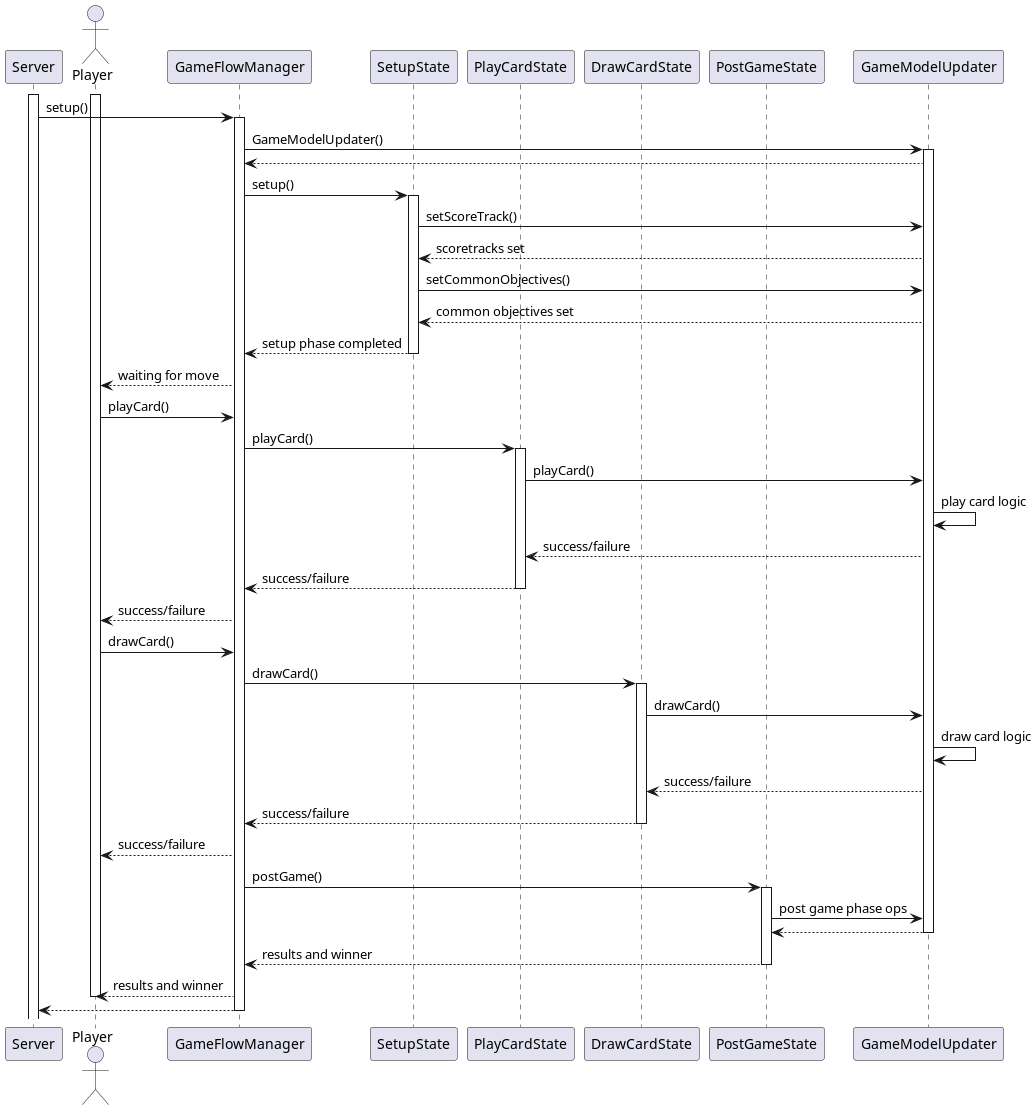
\includegraphics[scale=0.27]{pngs/sequence_controller}
\end{center}
\subsection{GameModelUpdater}
This class is the section of the controller whose logic allows to update the model, following players' moves.
More precisely, the more important methods are:
\begin{itemize}
    \item \texttt{playCard}: it allows a player to place a card on his board.
                             The method checks whether the player can play that card in that position and updates all structures accordingly.
    \item \texttt{drawPlayableCard}: this method is split in four sub-methods, one for each \texttt{Deck} type.
                              If the player is drawing from the visible card, an integer is required to discriminate which card he is selecting.
    \item \texttt{drawObjectiveCard}: used in the setup phase by the \texttt{GameFlowManager}.
    \item \texttt{drawStarterCard}: used in the setup phase by the \texttt{GameFlowManager}.
\end{itemize}

\subsection{Server}
The \texttt{Server} enum, implemented using the singleton pattern, is the module that contains all the lobbies and users logic.
It's implemented as an enum, so it can be called from anywhere using it's only value \texttt{Server.INSTANCE}.
Therefore, it doesn't have synchronization issues when constructing it and when retrieving the instance (that a static class would have).
\begin{center}
    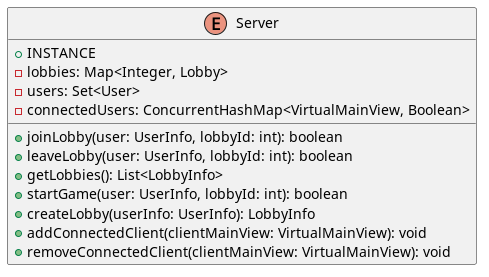
\includegraphics[scale=0.5]{pngs/server}
\end{center}
The server also keeps track of connected clients to send updates.
The collection used is a \texttt{Map} from \texttt{VirtualMainView} to \texttt{Boolean}, \texttt{true} when the user is not
in-game, so we know what clients should receive the main menu updates.


\end{document}